%%% D\'ebut du pr\'eambule %%%

%%%%%%%%%%%%%%%%%%%%%%%%%%%%%%%%%
% Options g\'en\'erales du document %
%%%%%%%%%%%%%%%%%%%%%%%%%%%%%%%%%

\documentclass[12pt]{report}	% Classe du document

%%%%%%%%%%%
% Langues %
%%%%%%%%%%%

\usepackage[english]{babel}		% Francisation de LaTeX

%%%%%%%%%%%%%%%%%%%%%%%
% Encodage, fontes... %
%%%%%%%%%%%%%%%%%%%%%%%

\usepackage[T1]{fontenc}
\usepackage[latin9]{inputenc}
\usepackage{amssymb}

\usepackage{latexsym}
\usepackage{amsmath,bm}
%\usepackage{graphicx}
\usepackage{aeguill}
\usepackage{aecompl}
\usepackage{url}
\usepackage{scribe_MG}
\usepackage{float}
\usepackage{graphicx}
\usepackage{caption}
\usepackage{subcaption}
%\usepackage{MnSymbol}
%\usepackage[lite]{mtpro2}
 		% Encodage d'entr\'ee : permet l'utilisation de caract\`eres accentu\'es en entr\'ee


\usepackage{graphicx}			% pour les images
\usepackage{float}
%%% Fin du pr\'eambule %%%
\def\ts{\top}
\def\XX{\mathbf{X}}
\def\wb{\mathbf{w}}
\def\xb{\mathbf{x}}
\def\yb{\mathbf{y}}
\def\db{\mathbf{d}}
\def\hb{\mathbf{h}}
\def\Diag{\text{Diag}}

\def\etab{\boldsymbol \eta}

%%% D\'ebut du document %%%

\begin{document}
	 
\scribe{}
%%\lecturenumber{2}			% required, must be a number
\hwnumber{ 2 }			% required, must be a 
%%\lecturedate{October 10}		% required, omit year
\hwdate{ March 4, 2015}		% required, omit year

	
\maketitle

%	\underline{For your information}\\
%\BIT
%\item
%Email: 
%\url{shuyu.dong@polytechnique.edu}
%\EIT

\newcommand{\doth}[2]{\Braket{#1,#2}_{\mathcal{H}}}
\newcommand{\phixi}{\Phi(x_i)} 
%\newcommand{\argmin}{\arg\!\min}
%\newcommand{\argmax}{\arg\!\max}
\newcommand{\argmax}{\operatornamewithlimits{argmax}}
\newcommand{\normhh}[1]{\Vert #1 \Vert_{\mathcal{H}_K}^2}
\newcommand{\normh}[1]{\Vert #1 \Vert_{\mathcal{H}} }


\newcommand{\mc}[1]{\mathcal{#1} }
\newcommand{\mb}[1]{\mathbb{#1} }
\newcommand{\xin}[2]{#1_{#2} }
\newcommand{\sumi}[1]{\sum_{i=1}^n #1}
\newcommand{\sumij}[1]{\sum_{i,j=1}^n #1}
\newcommand{\sumj}[1]{\sum_{j=1}^p #1}

\newcommand{\twopartdef}[4]
{
	\left\{
		\begin{array}{ll}
			#1 & \mbox{if } #2 \\
			#3 & \mbox{ } #4
		\end{array}
	\right.
}

\newcommand{\abss}[1]{\vert #1\vert}

\newcommand{\espe}[1]{\mathbb{E}\Big[ #1 \Big]}
\newcommand{\espef}[2]{\mathbb{E}_{#1}\Big[ #2 \Big]}
\newcommand{\sumk}[1]{\sum_{k=1}^K #1}

\newcommand{\indi}[1]{\bm{1}_{\lbrace #1\rbrace }} 
\newcommand{\indib}[1]{\bm{1}_{C_{k'}}(X_{#1})} 

\newcommand{\xii}[1]{\xi_n^{(#1)}}
\newcommand{\hatpp}{\hat{p}_k^2}
\newcommand{\hatp}{\hat{p}_k}

\newcommand{\norminf}[1]{\Vert #1\Vert_{\infty}}
\newcommand{\norminff}[1]{\Vert #1\Vert_{\infty}^2}
\newcommand{\norme}[1]{\Vert #1\Vert_2}
\newcommand{\normee}[1]{\Vert #1\Vert_2^2}
\newcommand{\normees}[1]{\Vert #1\Vert_1}


\section{ Step 1 }


\section{ figures}


\begin{figure}[H]
        \centering
              \makebox[0.4\textwidth][c]{ \begin{subfigure}[b]{0.45\textwidth}
 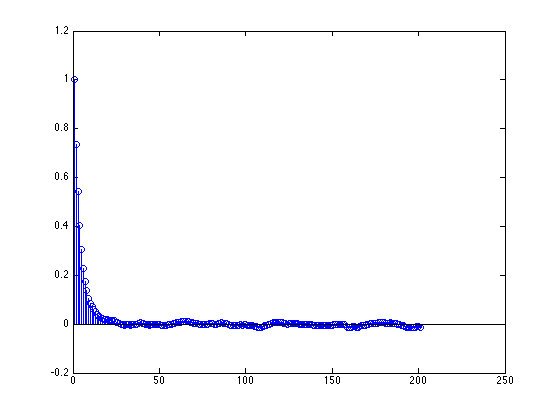
\includegraphics[width=\textwidth]{figures/ex3/4-acf-rw-quick}
%                \caption{Denoised images: d = 91. }
         %       \label{fig:1-real23}
        \end{subfigure}%
        \begin{subfigure}[b]{0.45\textwidth}
        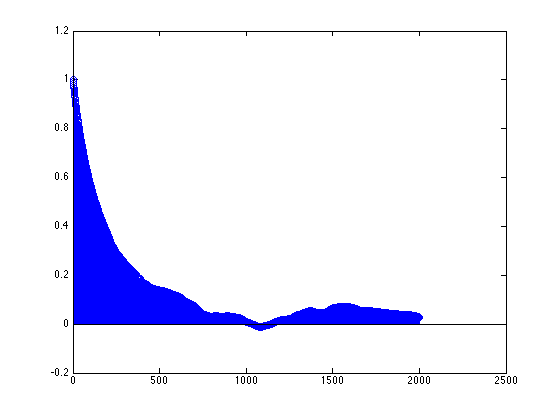
\includegraphics[width=\textwidth]{figures/ex3/4-acf-rw-slow}
%                \caption{ Denoised images: d = 115. }
                %\label{fig:1-real23}
        \end{subfigure}}
       \caption{\textbf{RW-MH: \texttt{sigma=1}(Left), \texttt{sigma=0.1}(Right):} correlograms of the markov chain of $10,000$ samples: when the variance parameter is smaller than an appropriate value, the convergence speed is much slower. }
\label{fig:1-reall23}
\end{figure} 


\begin{figure}[H]
\centering
\makebox[.4\textwidth][c]{         
 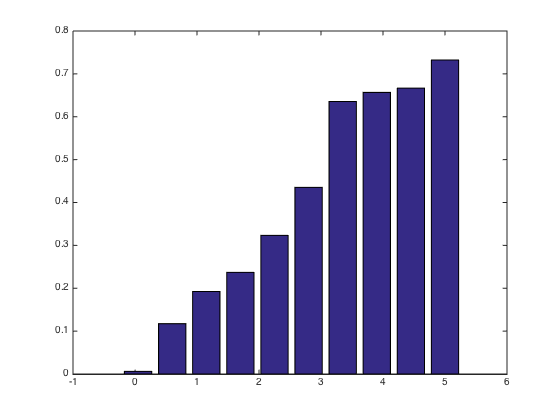
\includegraphics[width=0.6\textwidth]{figures/ex4/rel_error_sigma}
% \label{fig:orig}
 }
% \caption{\textbf{RDMH:} Correlogram of the markov chain $(X_n)$ of $10,000$ samples}
\label{fig:orig}
\end{figure} 






\end{document}
%%% Fin du document %%%
	
